
\medskip

Cet exercice est un questionnaire à choix multiples (QCM).

Aucune justification n’est demandée.

Pour chaque question, trois réponses (A, B et C) sont proposées.

\textbf{Une seule réponse est exacte.}

Recopier sur la copie le numéro de la question et la réponse.

\begin{center}
      \renewcommand{\arraystretch}{1.5}
  \begin{tabular}{|m{.55\textwidth}|>{\centering\arraybackslash}m{.14\textwidth}|>{\centering\arraybackslash}m{.14\textwidth}|>{\centering\arraybackslash}m{.14\textwidth}|}
  \hline
    \textbf{Questions} & \textbf{Réponse A} & \textbf{Réponse B} & \textbf{Réponse C} \\
   \hline
   %%%%%% question 1
   \textbf{1.} On considère les deux figures suivantes \par\vspace{0.25cm}
	Par quelle transformation la figure 2 est-elle l'image de la figure 1 ?\par \vspace{0.25cm}
\begin{center}
    	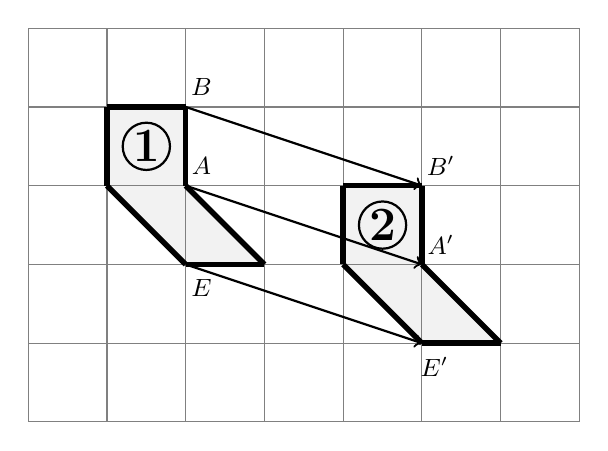
\begin{tikzpicture}[x=1cm,y=1cm]
\draw [color=gray,, xstep=1cm,ystep=1cm] (-4,-3) grid (3,2);
\clip(-4,-3) rectangle (3,2);
\fill[thick,color=gray,fill=gray,fill opacity=0.1] (-2,0) -- (-2,1) -- (-3,1) -- (-3,0) -- (-2,-1) -- (-1,-1) -- cycle;
\fill[thick,color=gray,fill=gray,fill opacity=0.1] (1,-1) -- (1,0) -- (0,0) -- (0,-1) -- (1,-2) -- (2,-2) -- cycle;
\draw [line width=2pt] (-2,0)-- (-2,1);
\draw [line width=2pt] (-2,1)-- (-3,1);
\draw [line width=2pt] (-3,1)-- (-3,0);
\draw [line width=2pt] (-3,0)-- (-2,-1);
\draw [line width=2pt] (-2,-1)-- (-1,-1);
\draw [line width=2pt] (-1,-1)-- (-2,0);
\draw [->,thick] (-2,1) -- (1,0);
\draw [line width=2pt] (1,-1)-- (1,0);
\draw [line width=2pt] (1,0)-- (0,0);
\draw [line width=2pt] (0,0)-- (0,-1);
\draw [line width=2pt] (0,-1)-- (1,-2);
\draw [line width=2pt] (1,-2)-- (2,-2);
\draw [line width=2pt] (2,-2)-- (1,-1);
\draw [->,thick] (-2,0) -- (1,-1);
\draw [->,thick] (-2,-1) -- (1,-2);
\begin{small}
\draw (-1.8,0.25) node {$A$};
\draw (-1.8,1.25) node {$B$};
\draw (-1.8,-1.3) node {$E$};
\draw (1.24,-0.75) node {$A'$};
\draw (1.24,0.25) node {$B'$};
\draw (1.16,-2.3) node {$E'$};
\end{small}
\draw [thick] (-2.5,0.5) circle (0.3);
\draw (-2.5,0.5) node {{\LARGE \textbf{1}}};
\draw [thick] (.5,-0.5) circle (0.3);
\draw (.5,-0.5) node {{\LARGE \textbf{2}}};
\end{tikzpicture}

    \end{center}    & Une translation & Une homothétie & Une symétrie axiale \\
   \hline
   %%%%%% question 2   
   \textbf{2.} On considère la représentation graphique de la fonction g suivante : \par\vspace{0.5cm}
\begin{center}
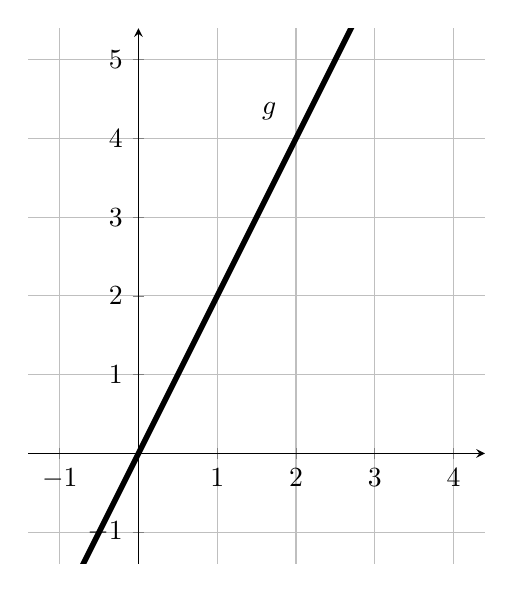
\begin{tikzpicture}[x=1cm,y=1cm]
\begin{axis}[
x=1cm,y=1cm,
axis lines=middle,
ymajorgrids=true,
xmajorgrids=true,
xmin=-1.4,
xmax=4.4,
ymin=-1.4,
ymax=5.4,
xtick={-1,0,...,4},
ytick={-1,-2,...,5},]
\clip(-2,-2) rectangle (4.5,5.5);
\draw [line width=2pt,domain=-2:4] plot(\x,{(-0--4*\x)/2});
\begin{scriptsize}
\draw[color=black] (1.66,4.34) node {$g$};
\end{scriptsize}
\end{axis}
\end{tikzpicture}
\end{center}   
Quel est l'antécédent de 2 par la fonction g ?   
    & 2 & 1 & 4\\
    \hline
\end{tabular}
\begin{tabular}{|m{.55\textwidth}|>{\centering\arraybackslash}m{.14\textwidth}|>{\centering\arraybackslash}m{.14\textwidth}|>{\centering\arraybackslash}m{.14\textwidth}|}
  \hline
    \textbf{Questions} & \textbf{Réponse A} & \textbf{Réponse B} & \textbf{Réponse C} \\
   \hline
    
    %%%%%% question 3
\textbf{3.} Soit f la fonction définie par : \par
$$ f : x \longmapsto 3x^2 -7$$
Quelle affirmation est correcte ?
& 29 est l'image de 2 par la fonction $f$.
& $f(3) = 20$
& $f$ est une fonction affine. \\ \hline     
    %%%%%% question 4
\textbf{4.} On a relevé les performances, en mètres, obtenues au
lancer du poids par un groupe de 13 élèves d’une classe.\par\vspace{0.25cm}
3,41 m ; 5,25 m ; 5,42 m ; 4,3 m ; 6,11 m ; 4,28 m ; 5,15 m ;\par 
3,7 m ; 6,07 m ; 5,82 m ; 4,62 m ; 4,91 m ; 4,01 m\par\vspace{0.25cm}
Quelle est la médiane de cette série de valeurs ?
& 7
& 4,91
& 5,15 \\ \hline     
    %%%%%% question 5
\textbf{5.} On considère la configuration suivante, dans laquelle les
triangles $LAC$ et $BUT$ sont semblables. \par 
\begin{center}
\begin{tikzpicture}[x=0.8cm,y=0.8cm]
\clip(-5.5,-3) rectangle (6,4.5);
\fill[thick,fill=white] (-4,4) -- (-5,3) -- (-2.5948249114601145,2.8245259404781935) -- cycle;
\fill[thick,fill=white] (0,2) -- (-3,-1) -- (4.2155252656196565,-1.5264221785654186) -- cycle;
\draw[thick] (-4,4)-- (-5,3);
\draw[thick] (-5,3)-- (-2.5948249114601145,2.8245259404781935);
\draw[thick] (-2.5948249114601145,2.8245259404781935)-- (-4,4);
\draw[thick] (0,2)-- (-3,-1);
\draw[thick] (-3,-1)-- (4.2155252656196565,-1.5264221785654186);
\draw[thick] (4.2155252656196565,-1.5264221785654186)-- (0,2);
\begin{scriptsize}
\draw (-5.4,4) node[anchor=north west] {$2,1 cm$};
\draw (-3.3,3.9) node[anchor=north west] {$2,4 cm$};
\draw (-4.1,2.9) node[anchor=north west] {$2,5 cm$};
\draw (-2.3,1.1) node[anchor=north west] {$6,3 cm$};
\draw (2,0.8) node[anchor=north west] {$7,2 cm$};
\draw (-0.1,-1.4) node[anchor=north west] {$7,5 cm$};
\draw (-4,4)-- ++(-2.5pt,-2.5pt) -- ++(5pt,5pt) ++(-5pt,0) -- ++(5pt,-5pt);
\draw (-3.9,4.3) node {$A$};
\draw (-5,3)-- ++(-2.5pt,-2.5pt) -- ++(5pt,5pt) ++(-5pt,0) -- ++(5pt,-5pt);
\draw (-5.2,2.7) node {$L$};
\draw (-2.6,2.8)-- ++(-2.5pt,-2.5pt) -- ++(5pt,5pt) ++(-5pt,0) -- ++(5pt,-5pt);
\draw (-2.3,2.8) node {$C$};
\draw (0,2)-- ++(-2.5pt,-2.5pt) -- ++(5pt,5pt) ++(-5pt,0) -- ++(5pt,-5pt);
\draw (0.1,2.3) node {$U$};
\draw (-3,-1)-- ++(-2.5pt,-2.5pt) -- ++(5pt,5pt) ++(-5pt,0) -- ++(5pt,-5pt);
\draw (-3.3,-1) node {$B$};
\draw (4.2,-1.5)-- ++(-2.5pt,-2.5pt) -- ++(5pt,5pt) ++(-5pt,0) -- ++(5pt,-5pt);
\draw (4.3,-1.2) node {$T$};
\end{scriptsize}
\end{tikzpicture}

\end{center}    
Par quel nombre doit-on multiplier l’aire du triangle $LAC$ pour
obtenir l’aire du triangle $BUT$ ?
& 3
& 6
& 9 \\ \hline     
  \end{tabular}
        \renewcommand{\arraystretch}{1}
\end{center}
\medskip

\clearpage
